% !TeX root = ../main.tex
% !TEX root = ../main.tex
% -*- root: ../main.tex -*-
% -*- program: pdflatex -*-
\chapter{双端修正}
上两章主要从插值方法和构造公式入手介绍了对~TOF~的~MRPC~的离线数据的刻度方法,研究的主要是单端的刻度。这章将介绍双端刻度方法。BESIII~实验的~MRPC~的读数条采用双端读出,因此对应一个事例双端共有两个信号值。可以利用两端信号值的均值进行刻度。

\begin{figure}[!h]
\begin{minipage}[!h]{0.5\linewidth}
%\centering
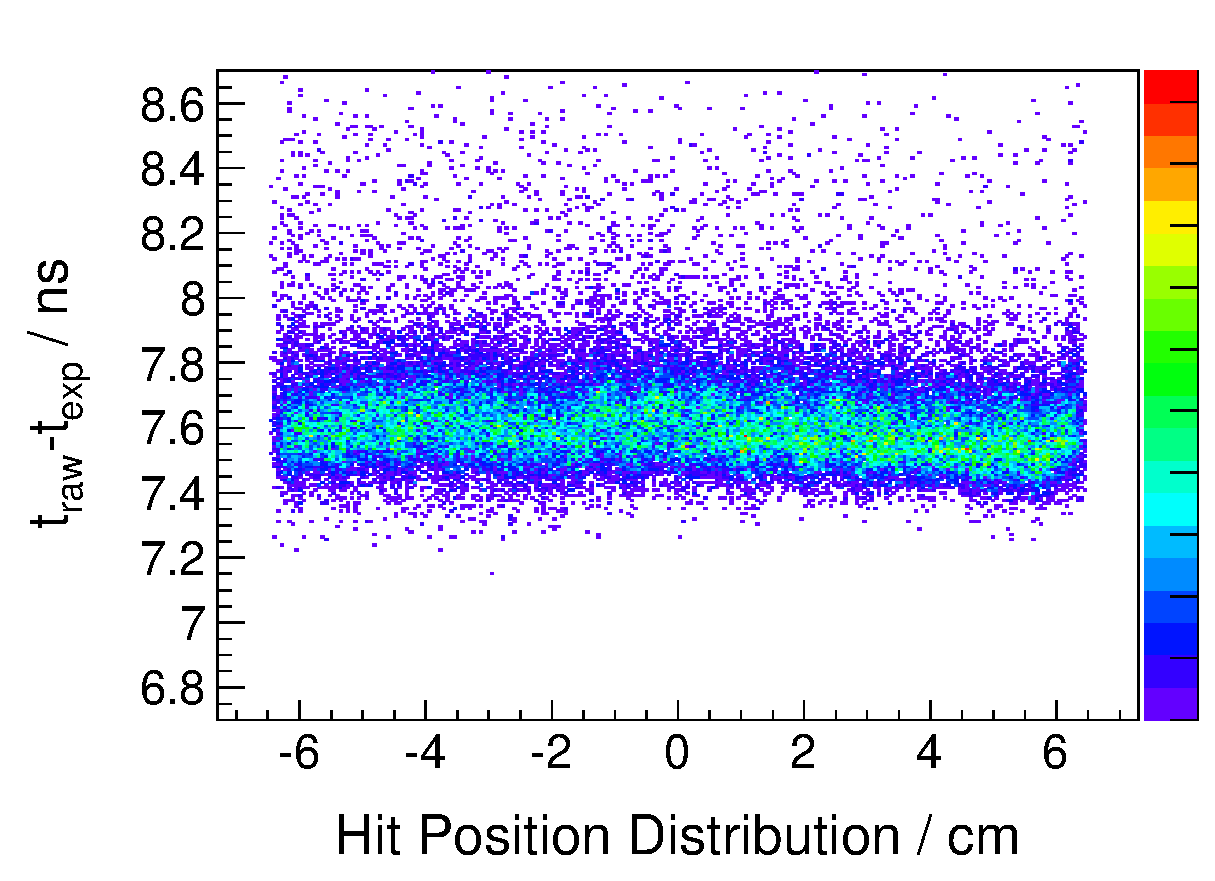
\includegraphics[width=0.9\textwidth]{chap4/combined-tVSz.eps}
\subcaption{双端时间对击中位置的分布}
\label{fig:combined-tVSz}
\end{minipage}%
\hfill
\begin{minipage}[!h]{0.5\linewidth}
%\centering
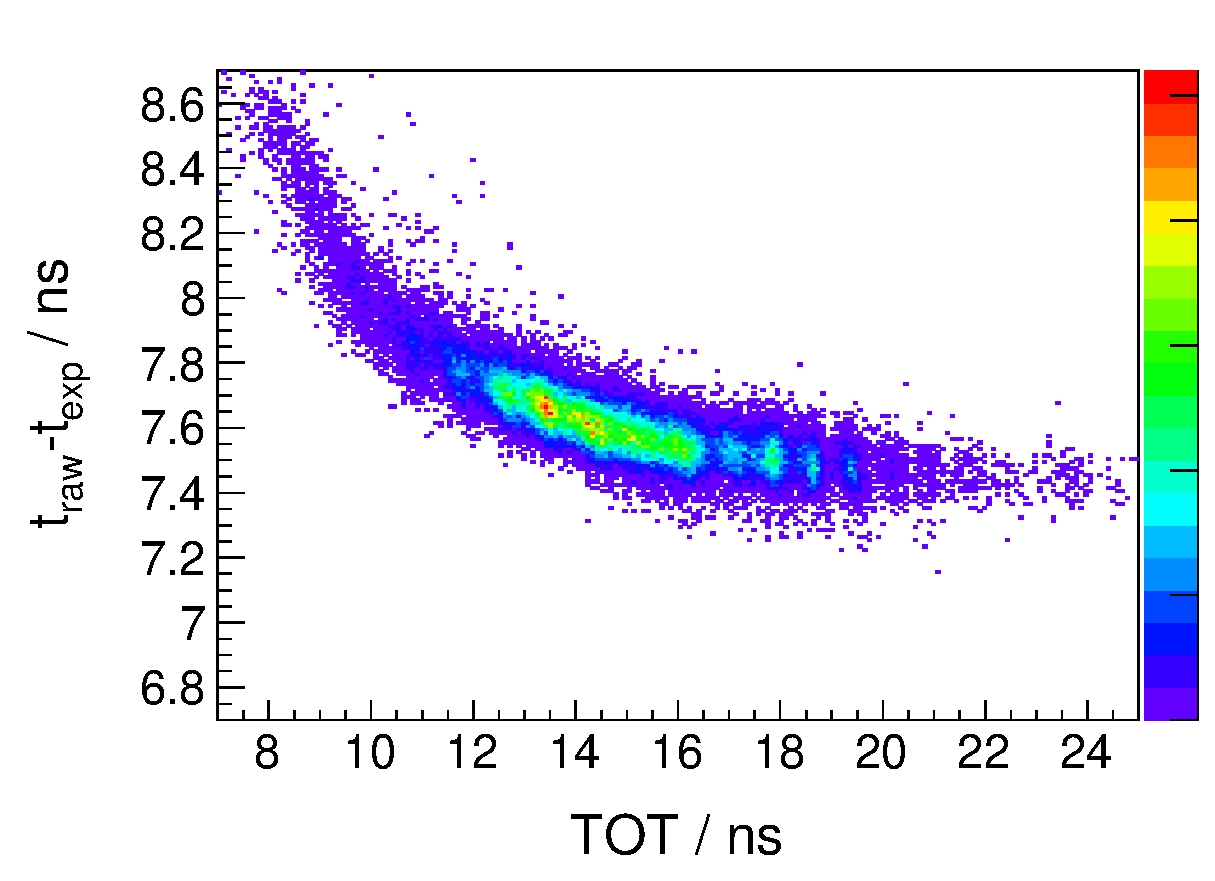
\includegraphics[width=0.9\textwidth]{chap4/combined-tVSq.eps}
\subcaption{时间对过阈时间的分布}
\label{fig:combined-tVSq}
\end{minipage}
\caption{双端时间对击中位置和过阈时间的分布}
\label{fig:combined}
\end{figure}

图~\ref{fig:combined}~是双端的时间对击中位置和过阈时间的分布。
%所谓双端指的是两端时间的平均值,过阈时间采用的也是两端过阈时间的平均值。
从图中可以看出,双端的时间对击中位置的依赖很小。时间对过阈时间的依赖关系和单端修正击中位置后时间对过阈时间的分布很类似。因此对于双端修正,直接对过阈时间修正,采用和单端修正击中位置后处理时间与过阈时间的关系相同的办法。

\section{双端插值方法}

\begin{figure}[!h]
\begin{minipage}[!h]{0.5\linewidth}
%\centering
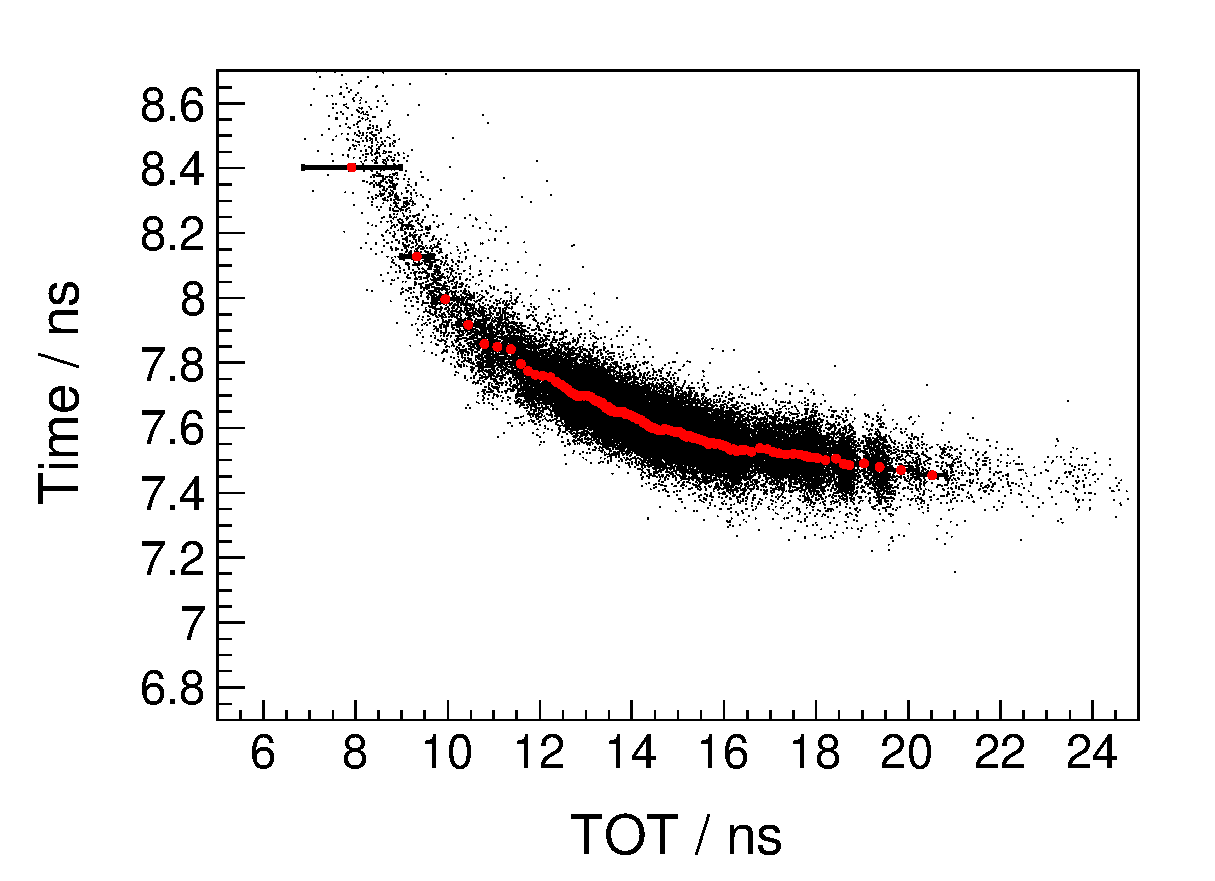
\includegraphics[width=0.9\textwidth]{chap4/combined-splines.eps}
\subcaption{双端插值}
\label{fig:combined-splines}
\end{minipage}%
\hfill
\begin{minipage}[!h]{0.5\linewidth}
%\centering
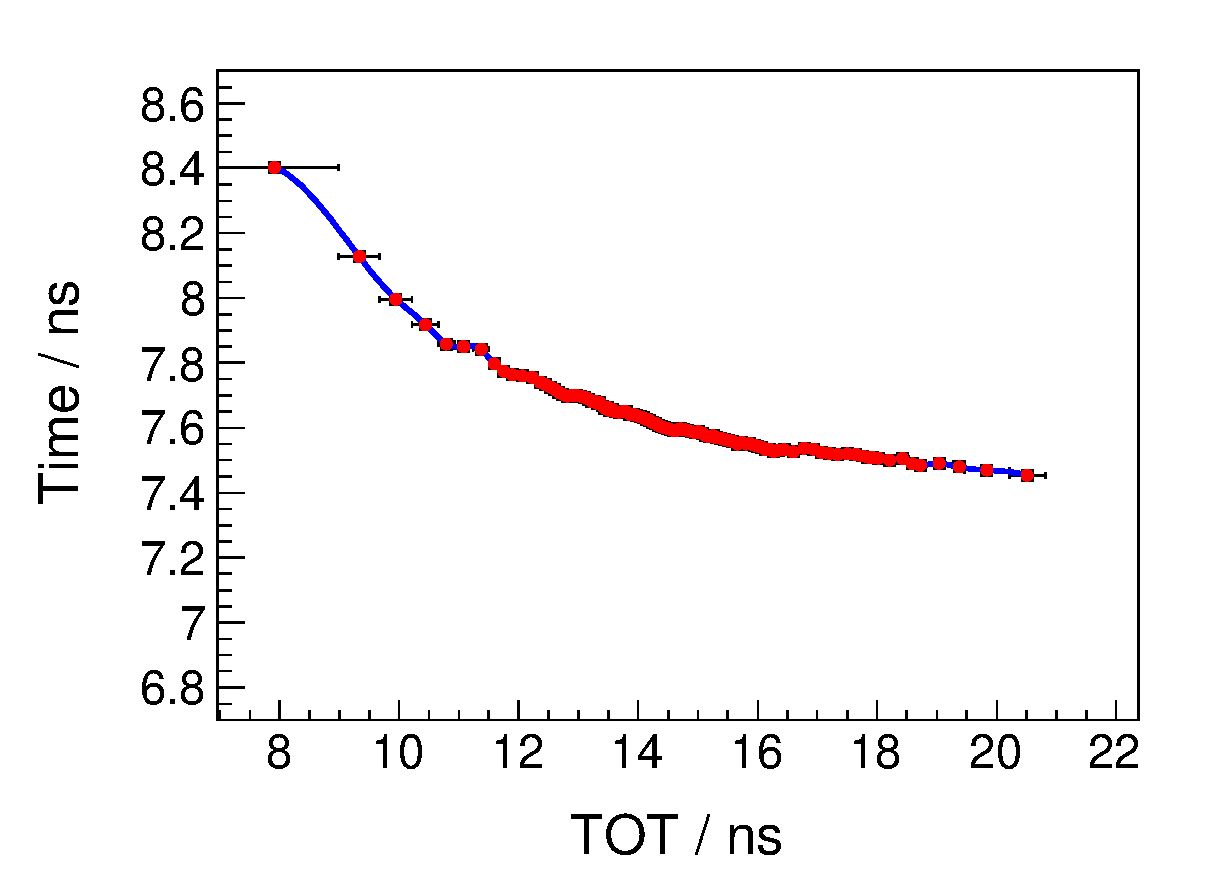
\includegraphics[width=0.9\textwidth]{chap4/combined-splines-line.eps}
\subcaption{双端插值线}
\label{fig:combined-splines-line}
\end{minipage}
\caption{双端插值方法}
\end{figure}

图~\ref{fig:combined-splines}~和图~\ref{fig:combined-splines-line}~表示的是双端的插值方法。图~\ref{fig:combined-splines}~采用的是和单端处理时间和过阈时间的一样的方法:将时间和过阈时间按过阈时间大小等事例数分成~100~份,对每个~bin~拟合得到中心值。图~\ref{fig:combined-splines-line}~表示的是对此~100~个点采用三阶样条插值拟合得到的曲线。

\section{双端构造公式}

图~\ref{fig:single-formula}~是上述几种公式拟合的结果。
就这一条的拟合结果来看,公式~\ref{eq:4}~,~\ref{eq:5}~拟合的比较符合。

\begin{figure}[!h]
\begin{minipage}{0.5\linewidth}
  \centerline{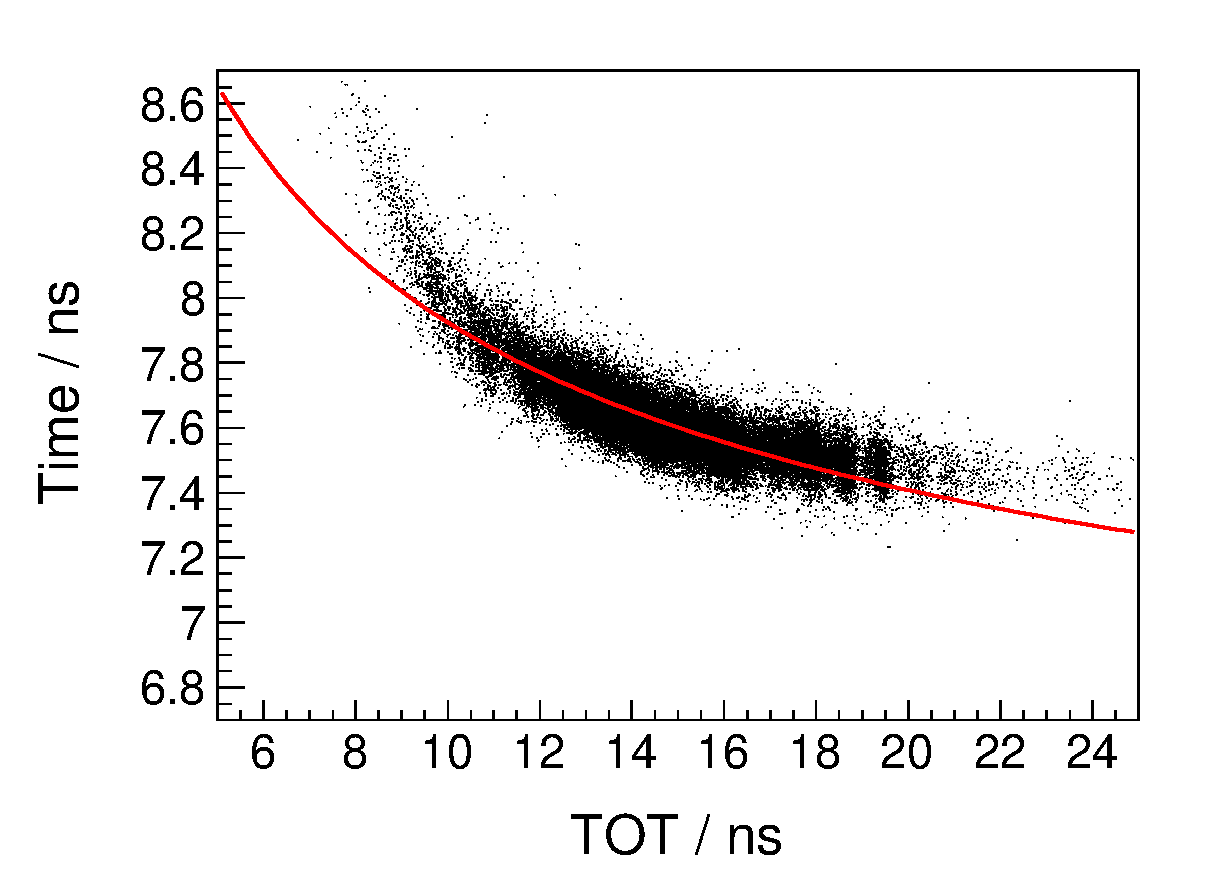
\includegraphics[width=0.9\textwidth]{chap4/double-half-order.eps}}
  \centerline{(a) 公式~\ref{eq:1}~的拟合}
  \centerline{\label{fig:double-half-order}}
\end{minipage}
\hfill
\begin{minipage}{0.5\linewidth}
  \centerline{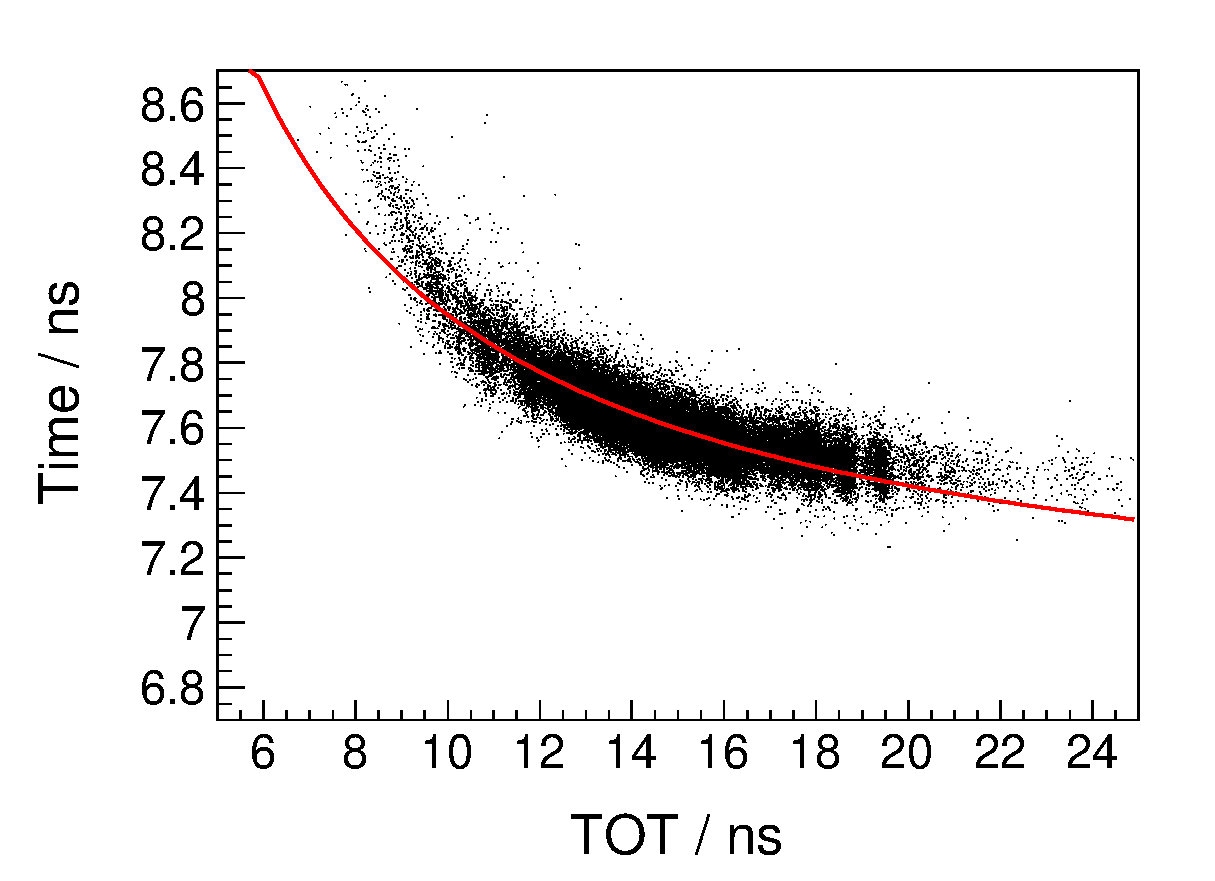
\includegraphics[width=0.9\textwidth]{chap4/double-1-order.eps}}
  \centerline{(b) 公式~\ref{eq:2}~的拟合}
  \centerline{\label{fig:double-1-order}}
\end{minipage}
\vfill
\begin{minipage}{0.5\linewidth}
  \centerline{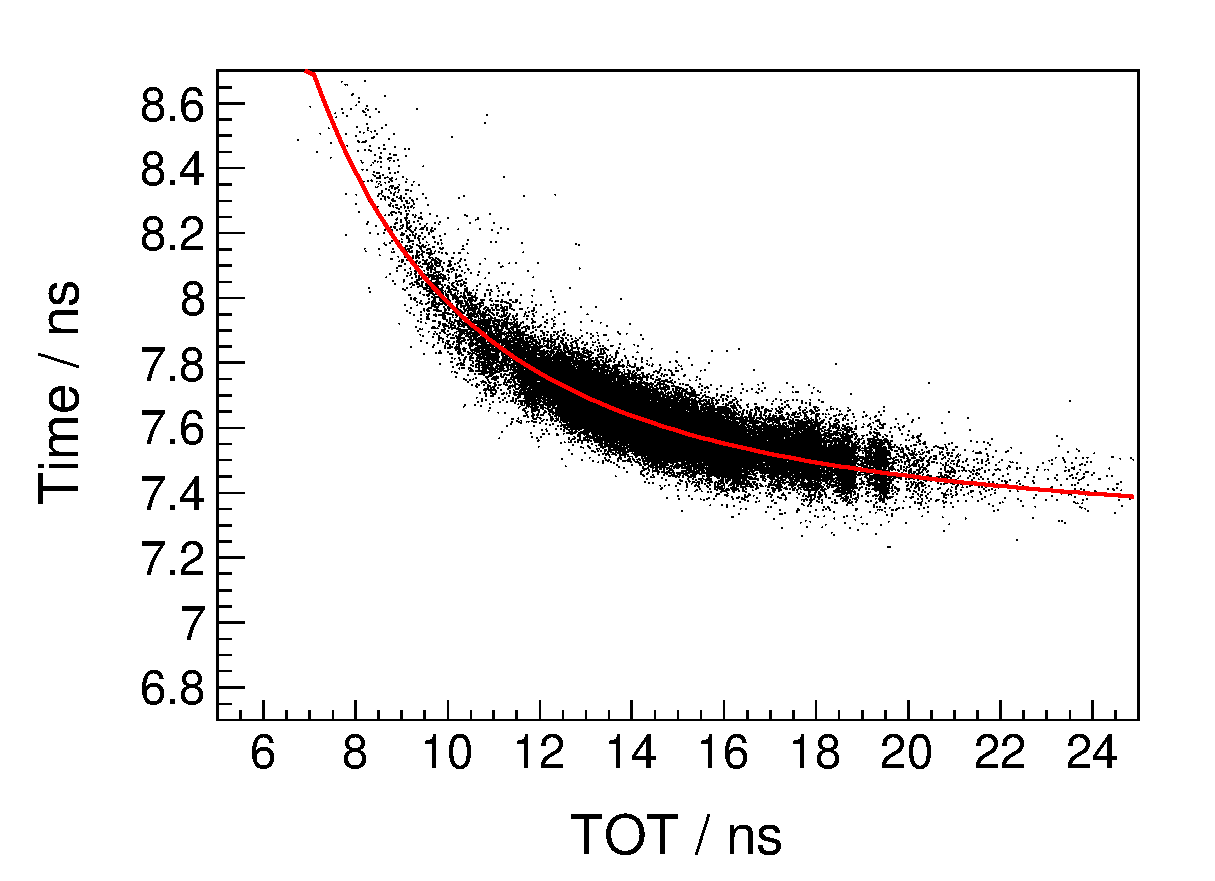
\includegraphics[width=0.9\textwidth]{chap4/double-2-order.eps}}
  \centerline{(c) 公式~\ref{eq:3}~的拟合}
  \centerline{\label{fig:double-2-order}}
\end{minipage}
\hfill
\begin{minipage}{0.5\linewidth}
  \centerline{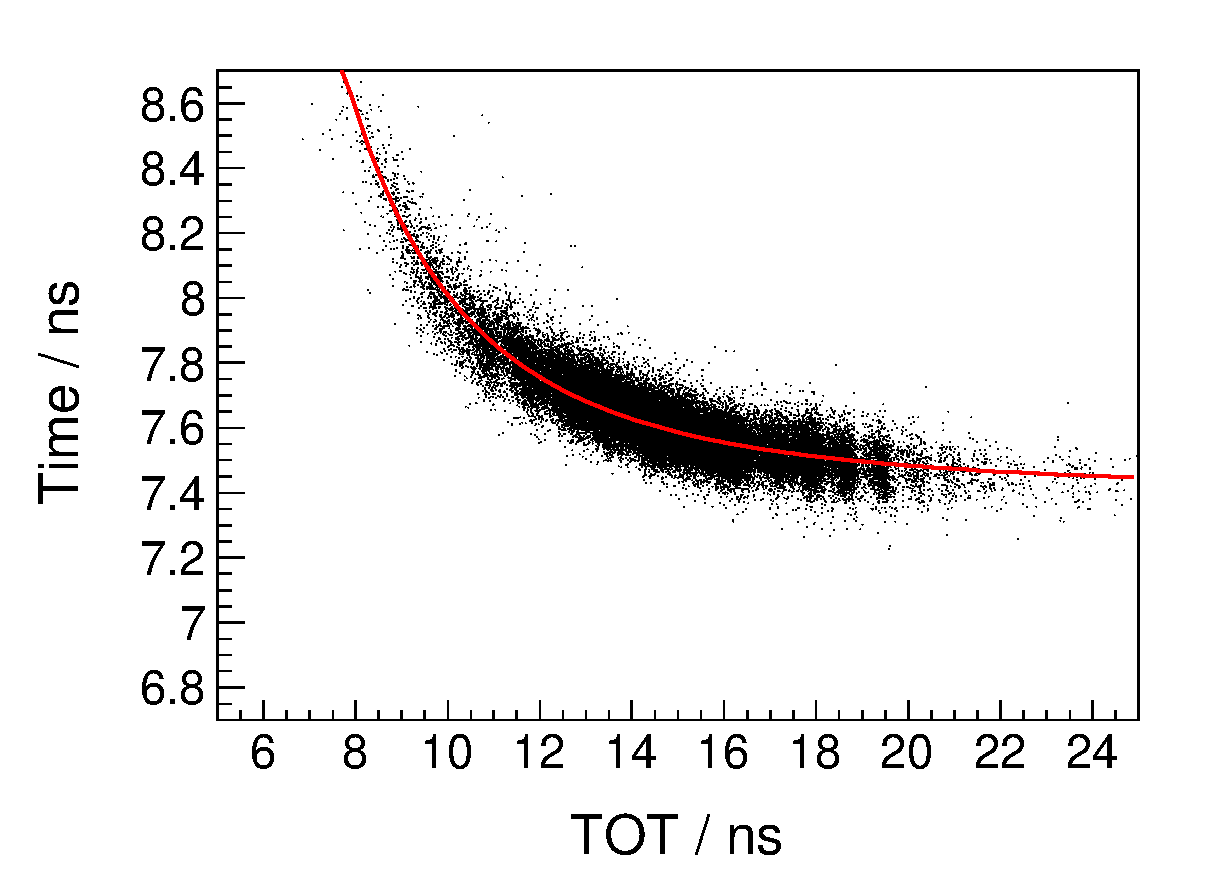
\includegraphics[width=0.9\textwidth]{chap4/double-3-order.eps}}
  \centerline{(d) 公式~\ref{eq:4}~的拟合}
  \centerline{\label{fig:double-3-order}}
\end{minipage}
\vfill
\begin{minipage}{0.5\linewidth}
  \centerline{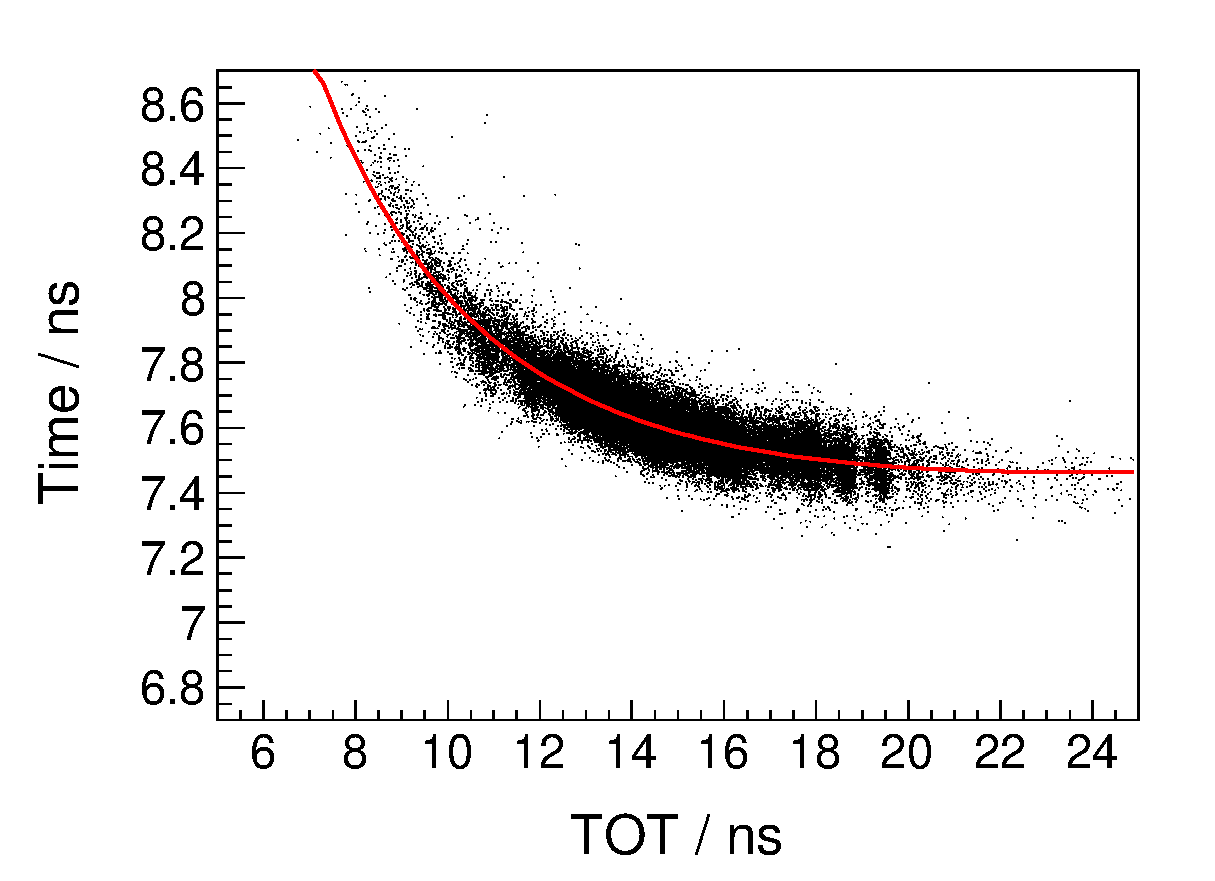
\includegraphics[width=0.9\textwidth]{chap4/double-half-1-order.eps}}
  \centerline{(e) 公式~\ref{eq:5}~的拟合}
  \centerline{\label{fig:double-half-1-order}}
\end{minipage}
\hfill
\begin{minipage}{0.5\linewidth}
  \centerline{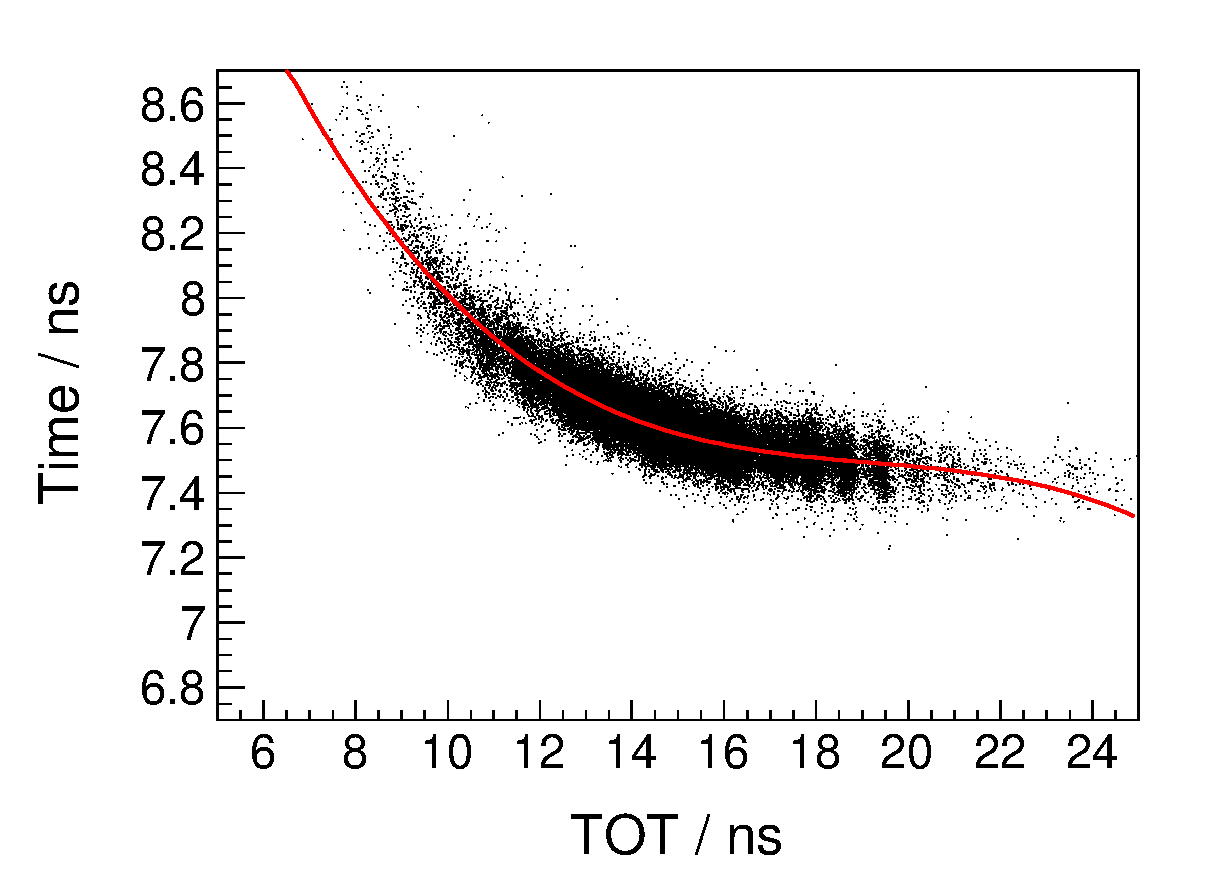
\includegraphics[width=0.9\textwidth]{chap4/double-pol3-order.eps}}
  \centerline{(f) 公式~\ref{eq:6}~的拟合}
  \centerline{\label{fig:double-pol3-order}}
\end{minipage}
\caption{几种公式对过阈时间的拟合}
\label{fig:single-formula}
\end{figure}

表~\ref{tbl:combined-resolution}~给出了这几种公式修正完成后得到的时间分辨。可以看出公式${p_{0}+p_{1}/\sqrt{q}+p_{2}/q}$的结果是最好的。

在此研究的基础上随机选了两个模块,然后比较几种公式修正得到的时间分辨的。见图~\ref{fig:double-module45}~和图~\ref{fig:double-module50}~。可以看出,除了使用多项式外,公式${p_{0}+p_{1}/\sqrt{q}+p_{2}/q}$得到的时间分辨基本是最好的。

\begin{table}[h]
    \centering
    \caption{\label{tbl:combined-resolution} 各种公式修正后时间分辨}
  \footnotesize
    \begin{tabular}{lc}
        \hline
        公式& 时间分辨(ps) \\
        \hline
        ${p_{0}+p_{1}/\sqrt{q}}$ & 60.1 \\
        ${p_{0}+p_{1}/q}$ & 58.9 \\
        ${p_{0}+p_{1}/q^{2}}$ & 65.9 \\
        ${p_{0}+p_{1}/q^{3}}$ & 56.7 \\
        ${p_{0}+p_{1}/\sqrt{q}+p_{2}/q}$ & 56.4 \\
        ${p_{0}+p_{1}*q+p_{2}*q^{2}+p_{3}*q^3}$ & 56.6 \\
        spline-fit&   55.8 \\
        \hline
    \end{tabular}
\end{table}

\begin{figure}[!h]
\begin{minipage}[!h]{0.5\linewidth}
%\centering
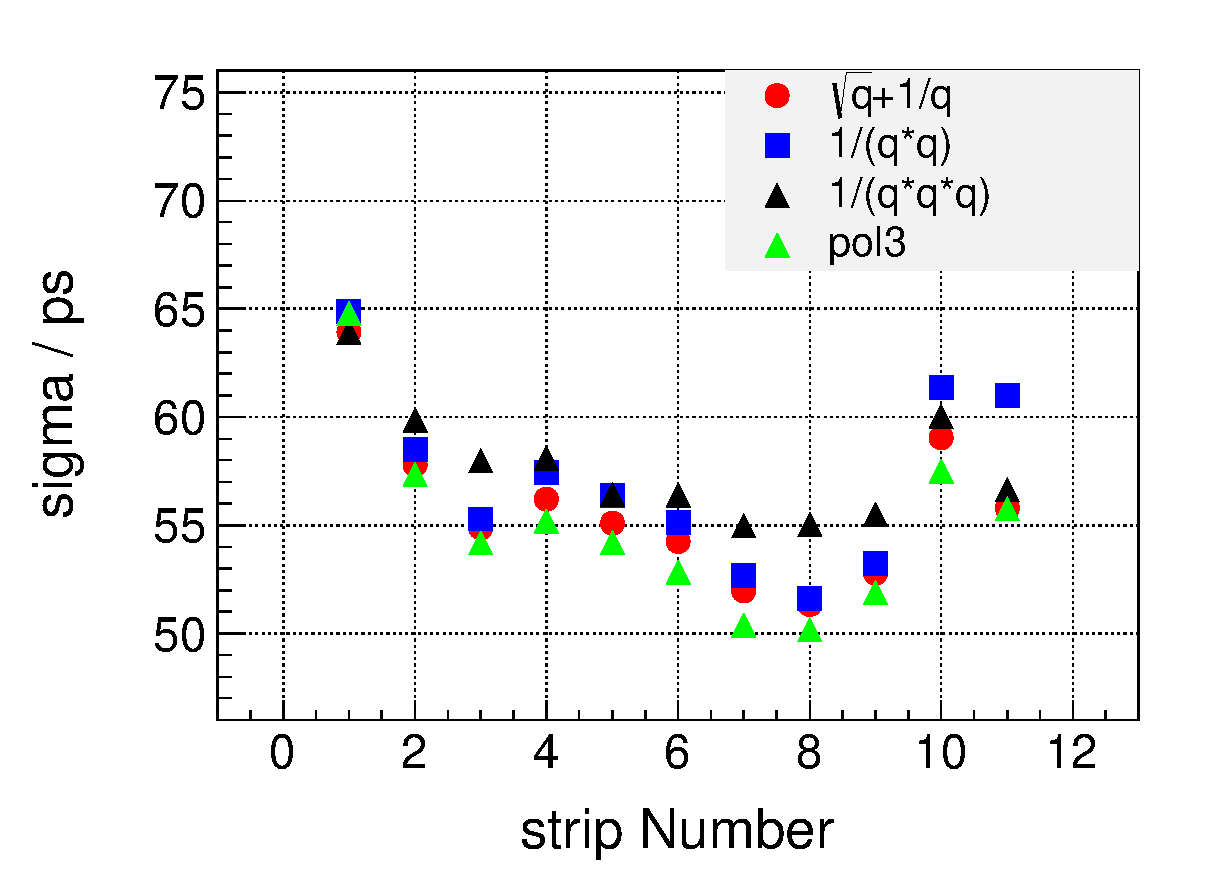
\includegraphics[width=0.9\textwidth]{chap4/double-module45.eps}
\subcaption{模块编号为45的几种公式时间分辨的比较}
\label{fig:double-module45}
\end{minipage}%
\hfill
\begin{minipage}[!h]{0.5\linewidth}
%\centering
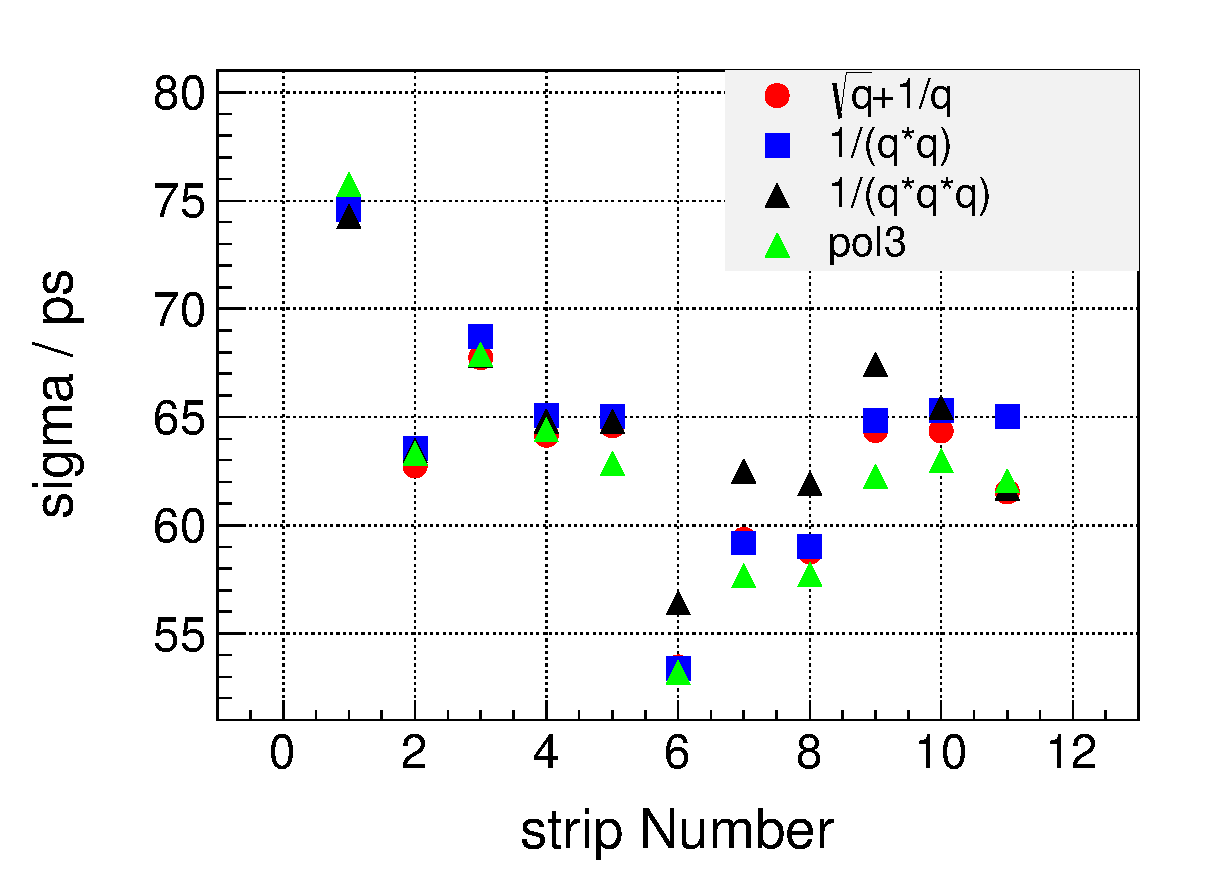
\includegraphics[width=0.9\textwidth]{chap4/double-module50.eps}
\subcaption{模块编号为50的几种公式时间分辨的比较}
\label{fig:double-module50}
\end{minipage}
\caption{几种公式修正得到的时间分辨的比较}
\end{figure}

\begin{figure}[!h]
\begin{minipage}[!h]{0.5\linewidth}
%\centering
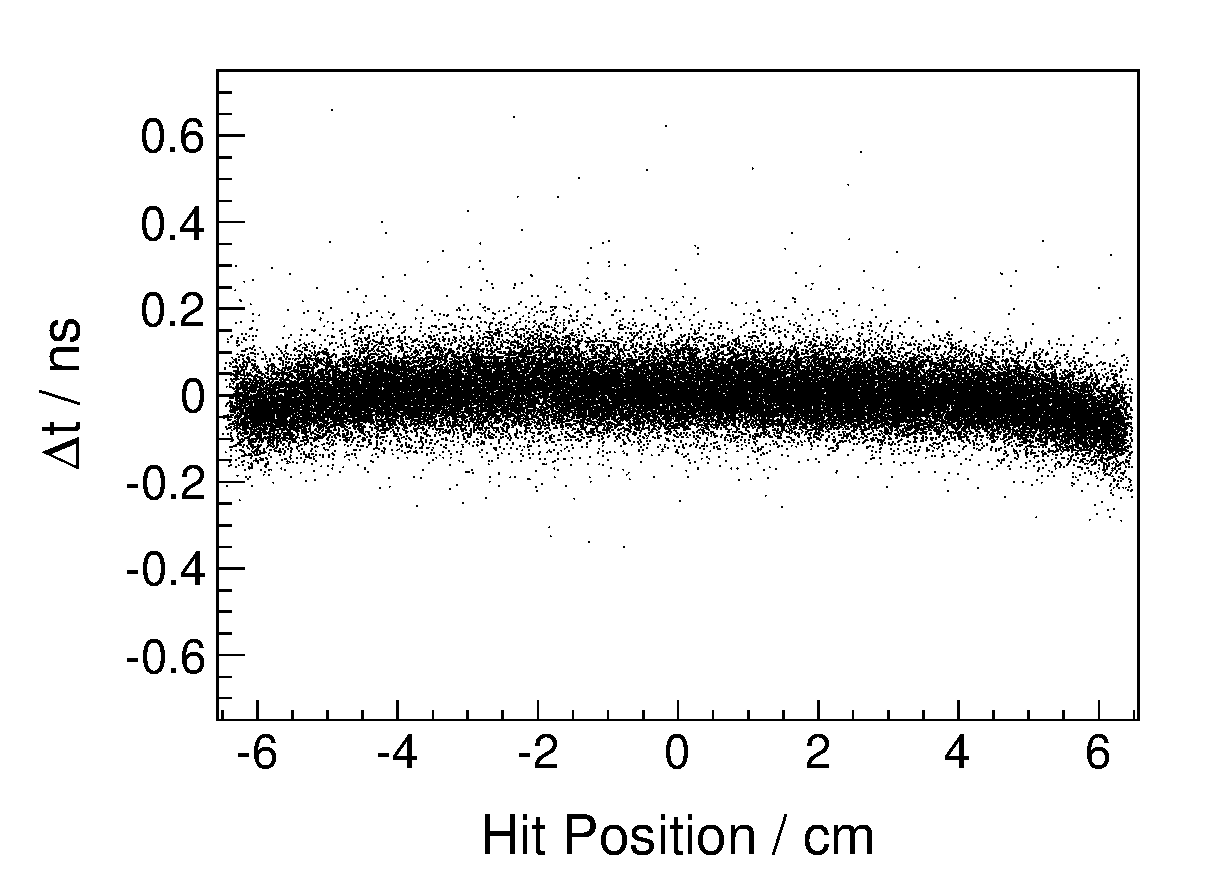
\includegraphics[width=0.9\textwidth]{chap4/Form-tVSz1.eps}
\subcaption{双端修正过阈时间后时间对击中位置的分布}
\label{fig:Form-tVSz1}
\end{minipage}%
\hfill
\begin{minipage}[!h]{0.5\linewidth}
%\centering
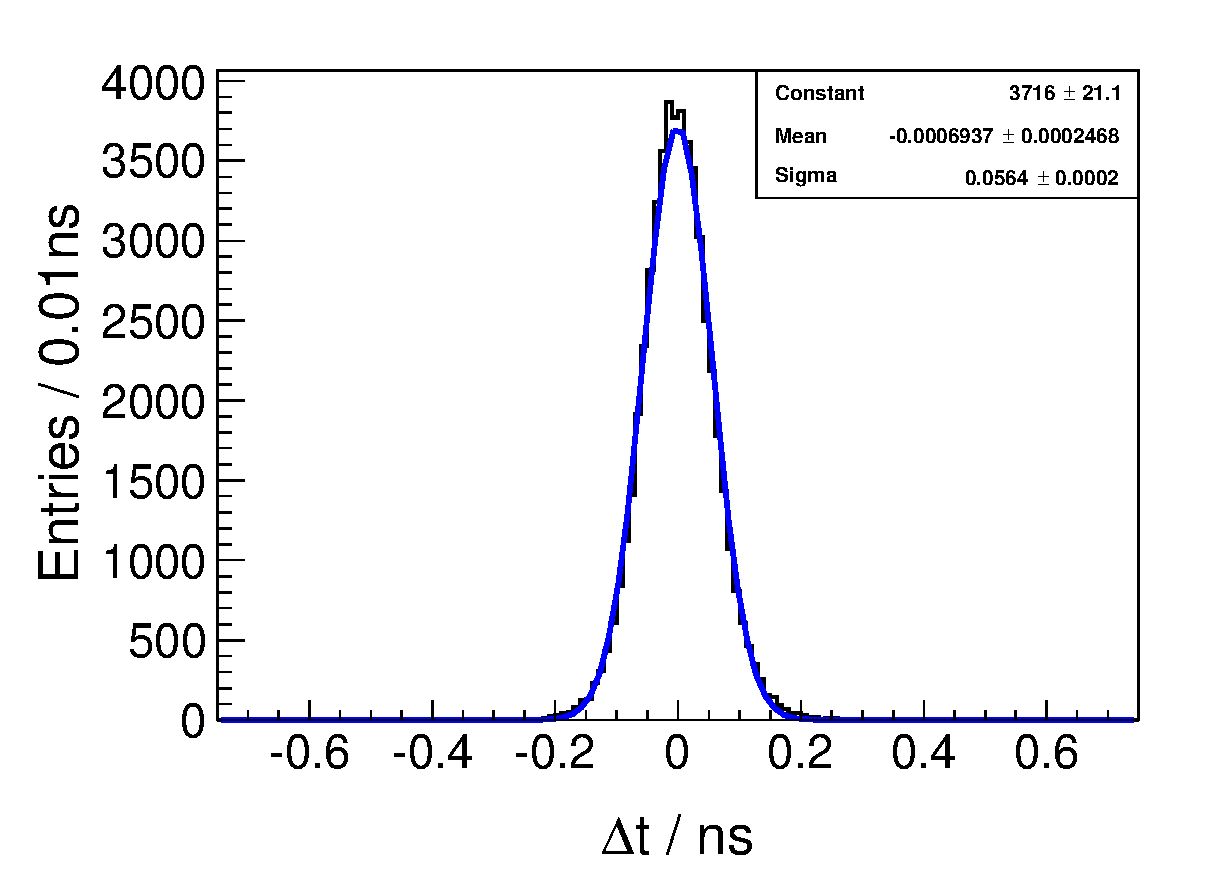
\includegraphics[width=0.9\textwidth]{chap4/Form-sigma1.eps}
\subcaption{双端修正过阈时间后的时间分辨}
\label{fig:Form-sigma1}
\end{minipage}
\caption{双端修正过阈时间后的分布}
\end{figure}

\section{双端对击中位置的修正}

图~\ref{fig:Form-tVSz1}~给出了双端时间修正过阈时间后时间对击中位置的分布,可以看出还是有一定的依赖。对此需要对击中位置击中位置进行修正。

%%这部分需要写完前面的径迹外推后再写。
在第二章中讲到重建流程时指出击中位置(zrhit)来自于径迹外推。在读数条边界处会有偏差。为了避开使用击中位置的信息,选择使用和它类似的信息量~($t_{left}$-$t_{right}$)/2~代替它。
~$t_{left}$=(L+zrhit)/v+$C_{0}$~;
$t_{right}$=(L-zrhit)/v+$C_{1}$~
两式相减除2得~($t_{left}$-$t_{right}$)/2=zrhit/v+$C_{2}$~
定义~$t_{sub}$=($t_{left}$-$t_{right}$)/2~
其中~L~为半个读数条长,为一常量;~v~为信号在读数条内的传播速度,为常量;~$C_{0}$,$C_{1}$~分别是两端的时延等信息,为常量。~$C_{2}$=$C_{0}$-$C_{1}$~;综上得出~($t_{left}$-$t_{right}$)/2~与击中位置成正相关。

图~\ref{fig:zVStsub}~是~$t_{sub}$~和击中位置的分布,可以看出呈线性关系。
\begin{figure}[!h]
\centering
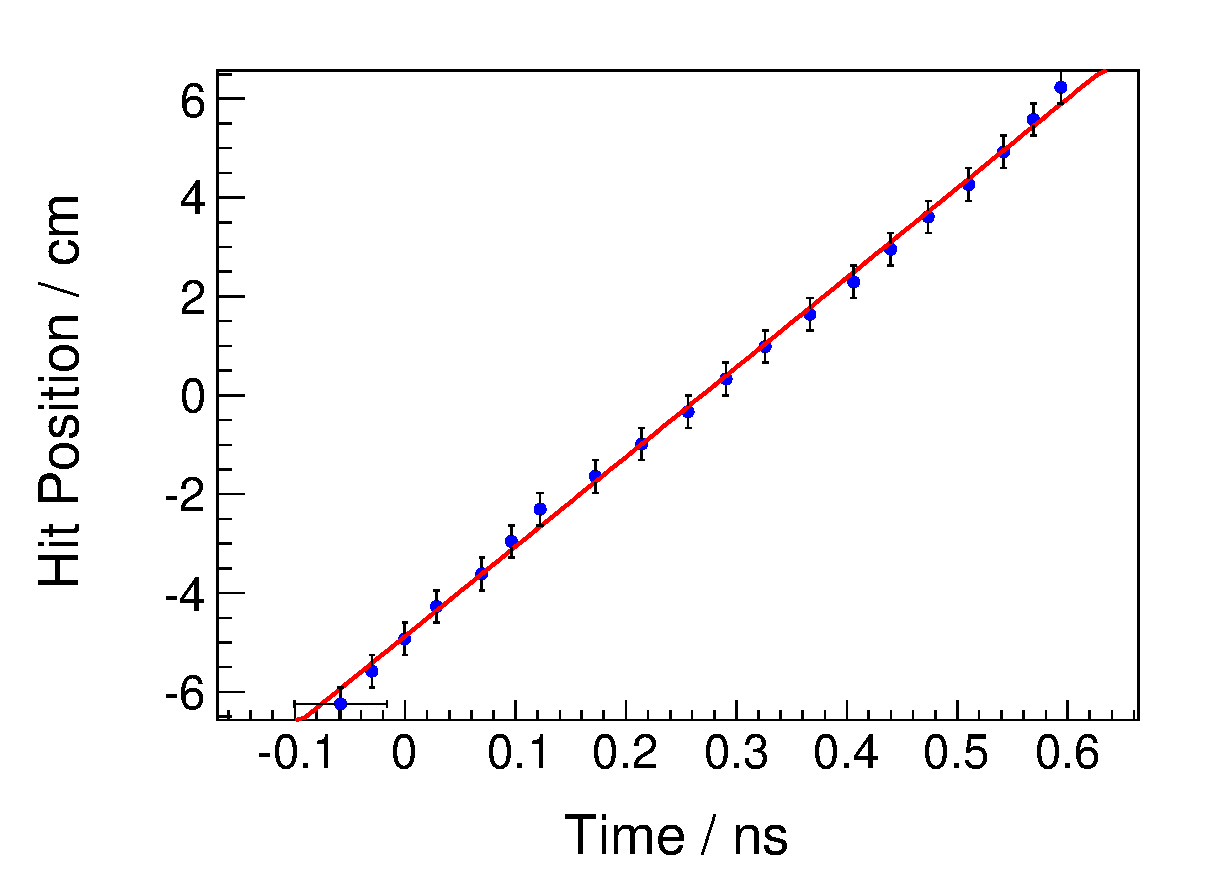
\includegraphics[width=0.6\textwidth]{chap4/zVStsub.eps}
\caption{击中位置与~($t_{left}$-$t_{right}$)/2~的分布}
\label{fig:zVStsub}
\end{figure}

基于此,可以利用$t_{sub}$信息修正击中位置。

\begin{figure}[!h]
\centering
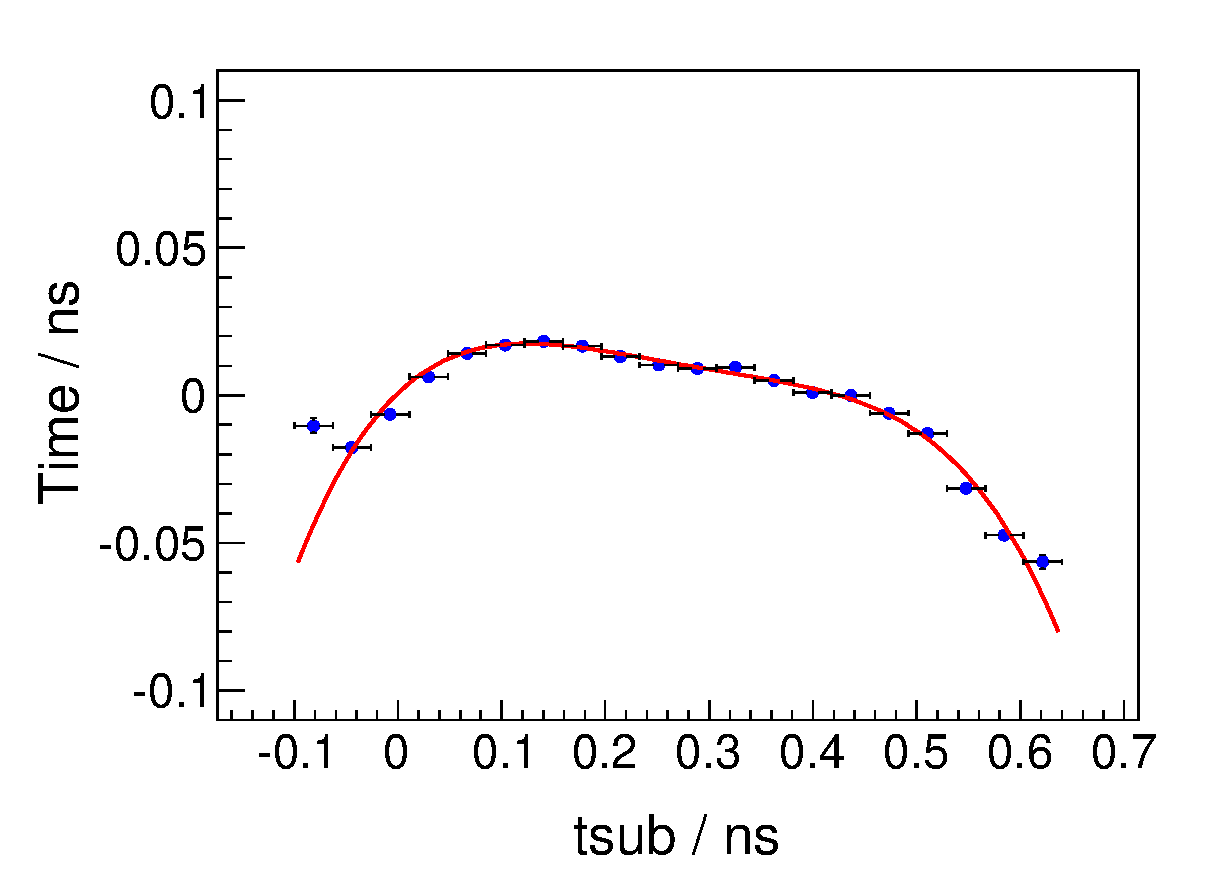
\includegraphics[width=0.6\textwidth]{chap4/Form-Fit-Tsub.eps}
\caption{对~$t_{sub}$~采用四阶多项式拟合}
\label{fig:Form-Fit-Tsub}
\end{figure}

图~\ref{fig:Form-Fit-Tsub}~是时间对~$t_{sub}$~的分布关系,对此采用了一个四阶多项式的修正。

图~\ref{fig:Fit-Tsub}~是修正~$t_{sub}$~前后,时间对~$t_{sub}$~和击中位置的分布关系。可以看出,修正过~$t_{sub}$~后,时间对击中位置的分布不再有明显的依赖。
\begin{figure}[!h]
\begin{minipage}{0.5\linewidth}
  \centerline{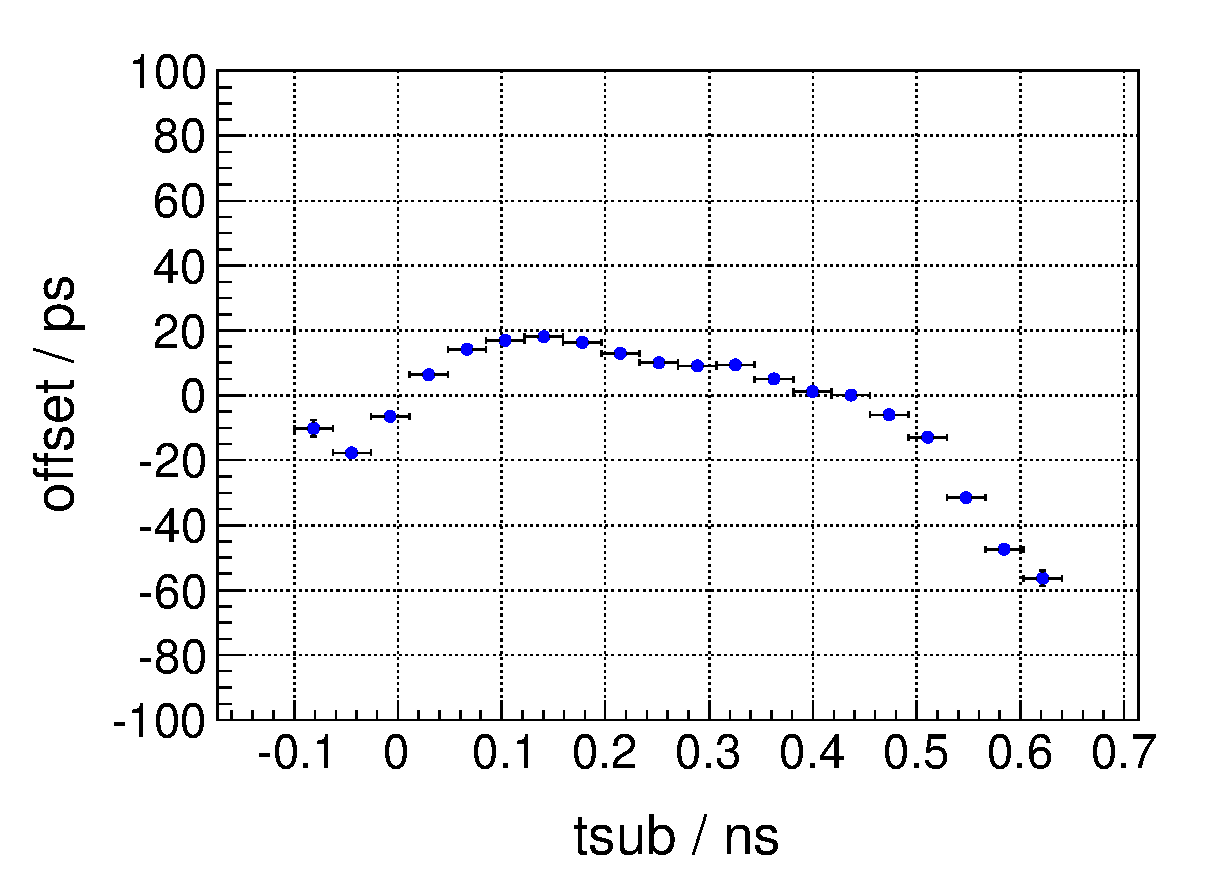
\includegraphics[width=0.9\textwidth]{chap4/before-offset-tsub.eps}}
  \centerline{(a) ~$t_{sub}$~修正前时间对~$t_{sub}$~的分布}
  \centerline{\label{fig:before-offset-tsub}}
\end{minipage}
\hfill
\begin{minipage}{0.5\linewidth}
  \centerline{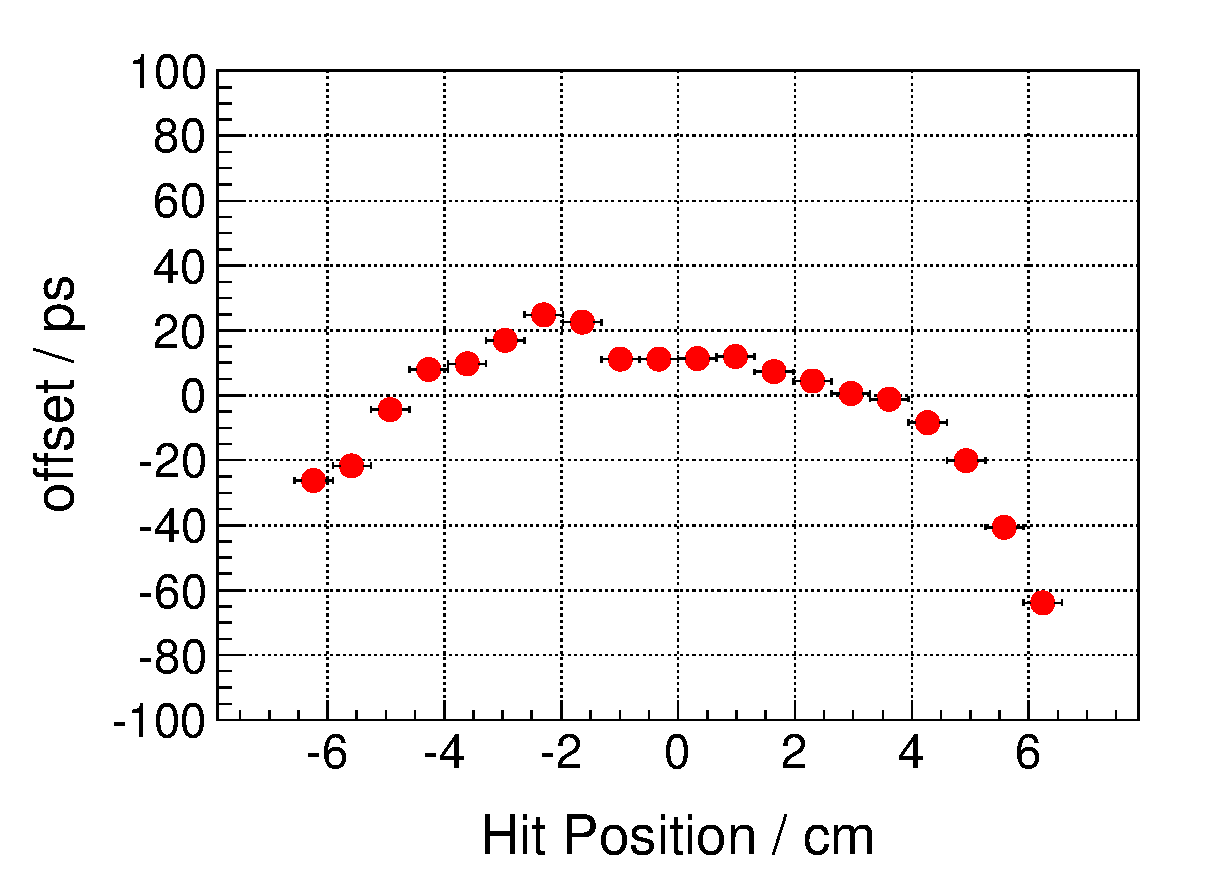
\includegraphics[width=0.9\textwidth]{chap4/before-offset-z.eps}}
  \centerline{(b) ~$t_{sub}$~修正前时间对击中位置的分布}
  \centerline{\label{fig:before-offset-z}}
\end{minipage}
\vfill
\begin{minipage}{0.5\linewidth}
  \centerline{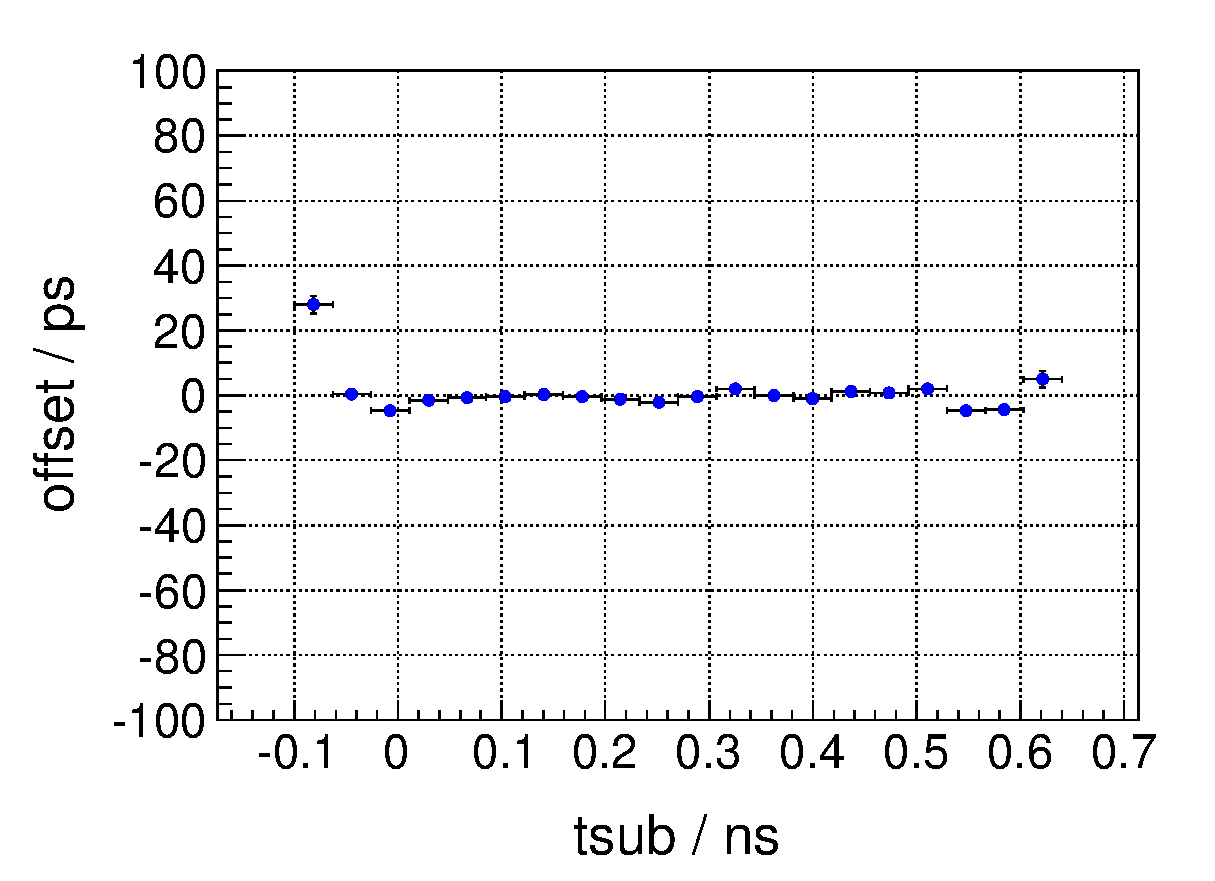
\includegraphics[width=0.9\textwidth]{chap4/after-offset-tsub.eps}}
  \centerline{(c) ~$t_{sub}$~修正后时间对~$t_{sub}$~的分布}
  \centerline{\label{fig:after-offset-tsub}}
\end{minipage}
\hfill
\begin{minipage}{0.5\linewidth}
  \centerline{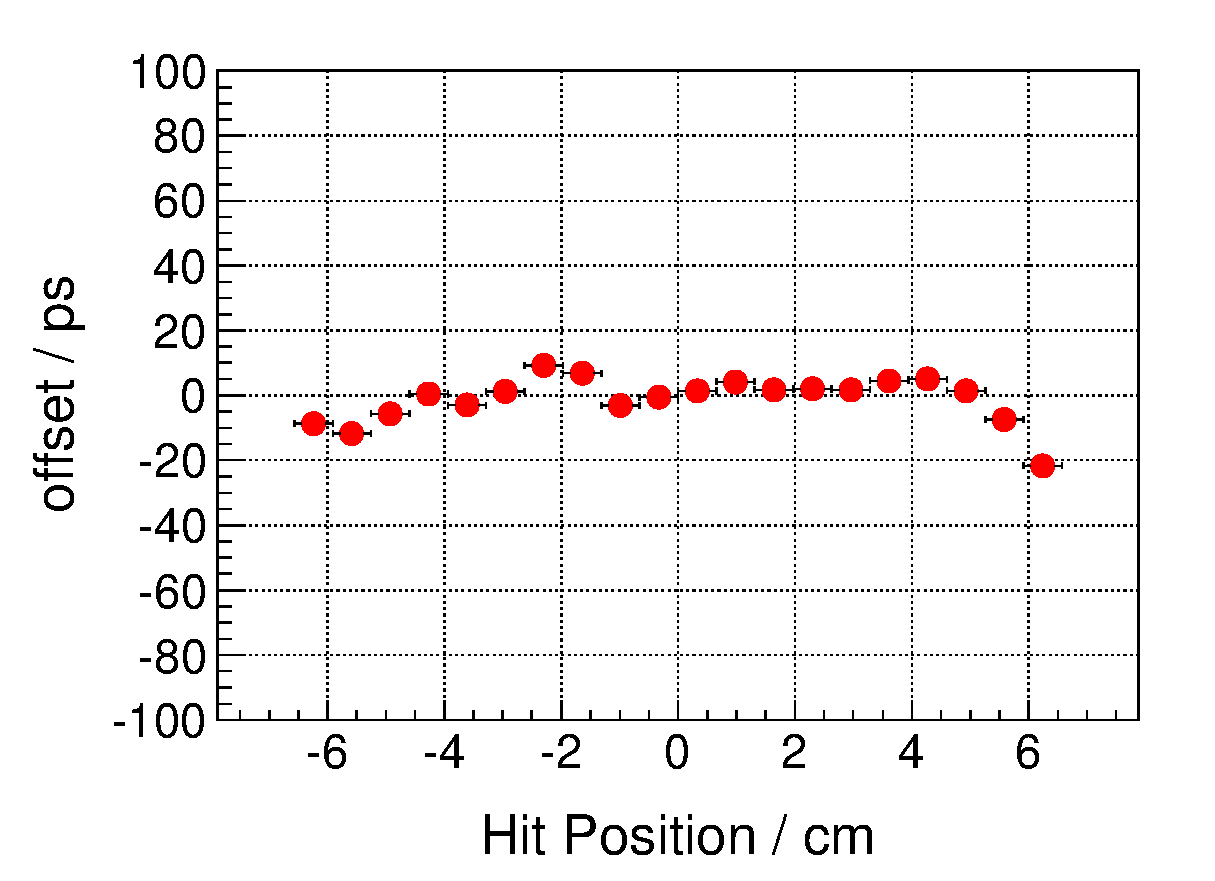
\includegraphics[width=0.9\textwidth]{chap4/after-offset-z.eps}}
  \centerline{(d) ~$t_{sub}$~修正后时间对击中位置的分布}
  \centerline{\label{fig:after-offset-z}}
\end{minipage}
\caption{~$t_{sub}$~修正前后时间对~$t_{sub}$~和击中位置的分布}
\label{fig:Fit-Tsub}
\end{figure}

\begin{figure}[!h]
\begin{minipage}[!h]{0.5\linewidth}
%\centering
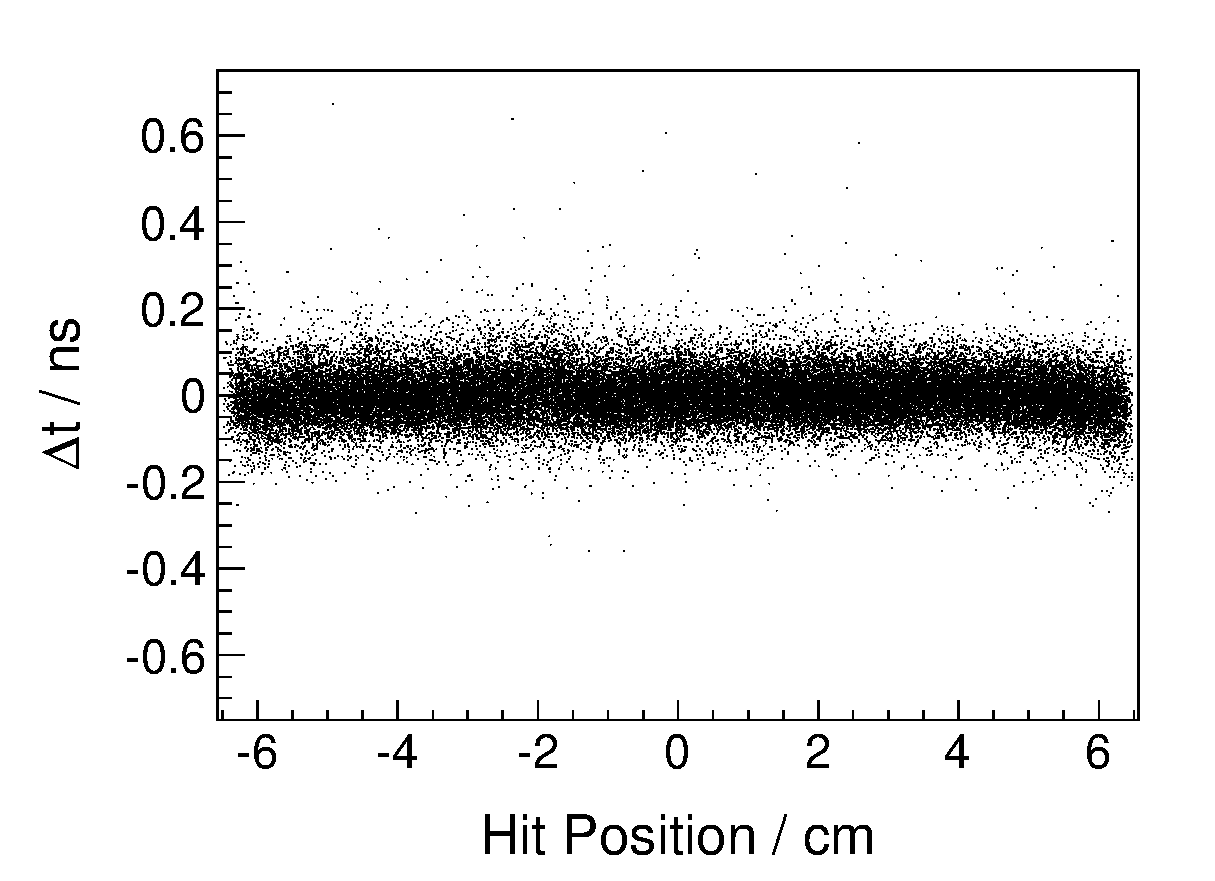
\includegraphics[width=0.9\textwidth]{chap4/Form-tVSz2.eps}
\subcaption{双端修正~$t_{sub}$~后时间对击中位置的分布}
\label{fig:Form-tVSz2}
\end{minipage}%
\hfill
\begin{minipage}[!h]{0.5\linewidth}
%\centering
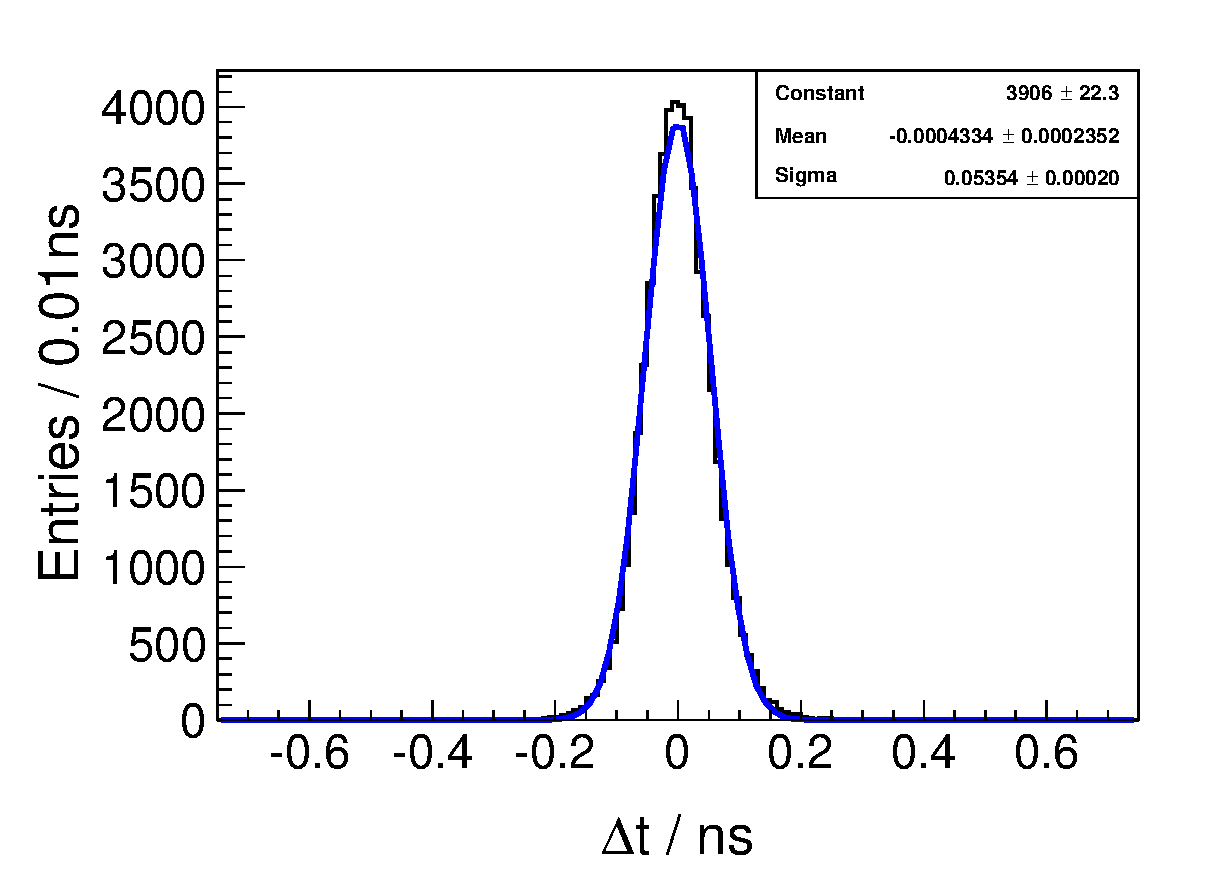
\includegraphics[width=0.9\textwidth]{chap4/Form-sigma2.eps}
\subcaption{双端修正~$t_{sub}$~后的时间分辨}
\label{fig:Form-sigma2}
\end{minipage}
\caption{双端修正~$t_{sub}$~后的分布}
\end{figure}

图~\ref{fig:Form-tVSz2}~是修正~$t_{sub}$~后时间对~击中位置~的分布的散点图。可以看出这时候分布关系已经基本平滑。图~\ref{fig:Form-sigma2}~是修正~$t_{sub}$~后双端的时间分辨,为~53.5~ps。相应的先对双端的过阈时间进行插值拟合修正后得到的时间分辨是~55.8~ps。插值修正过阈时间后,再对击中位置进行修正,得到的最终的时间分辨是~53.2~ps。

\section{小结}

本章介绍了双端刻度方法的研究。BESIII~实验的~MRPC-TOF~的读数条采取的是双端读出的方式,对应的一个事例在读数条两端各有信号测量值,采用两个测量值的均值进行刻度。这时的时间对击中位置的分布依赖很弱,而时间与过阈时间的分布和单端修正完击中位置后时间与过阈时间的分布类似。因此先对过阈时间进行修正,采用的是和单端对此修正一样的方法。修正完过阈时间后,发现时间对击中位置还是有些依赖的。考虑到由于边界效应,径迹外推得到的击中位置(zrhit)在读数条两端有偏差,而信息量~($t_{left}$-$t_{right}$)/2~和击中位置之间存在线性关系。因此采用了信息量~($t_{left}$-$t_{right}$)/2~对击中位置进行修正。最终得到双端的单条修正后的时间分辨为~53.5~ps。











